\chapter{Implementação}\label{cap:methods}

Neste capítulo, iremos explorar as ferramentas e métodos utilizados na
concepção de um ambiente robótico simulado para um manipulador com cinco graus
de liberdade do tipo 5R. O manipulador tem uma cadeia cinemática simples que
pode ser entendida como a composição de dois outros braços planares, mas que
permite que a posição do efetuador final não esteja limitada, por exemplo, a um
plano de altura constante. Começaremos explorando a modelagem da cadeia
cinemática e também a representação do modelo virtual do robô dentro do
simulador \emph{Webots}. Em seguida, iremos definir a arquitetura de
comunicação proposta para se controlar o manipulador utilizando o conceito de
\emph{Actions} presente no framework \emph{Robot Operating System} (ROS), o
qual permitiu uma implementação modularizada para execução dos experimentos.
Por fim, iremos detalhar o esquema de controle e bibliotecas utilizadas na
implementação do algoritmo \emph{Resolved Rate Control} para execução de
trajetórias retilíneas bem como os experimentos realizados para se avaliar a
resolução de redundância na execução de tais trajetórias.

\section{Simulação de manipuladores robóticos}

Simuladores de física tornam possível a pesquisa e desenvolvimento na robótica,
pois permitem que os pesquisadores testem e validem métodos teóricos
inicialmente ou exclusivamente em um simulador, uma vez que os robôs em si são
frequentemente caros, frágeis e escassos~\cite{robotic_applications}. Os
simuladores oferecem um ambiente acessível e barato de prototipação com uma
variedade de robôs disponíveis e prontos para uso, sem o risco de danificar o
equipamento físico economizando assim tempo e recursos. A simulação pode ser
executada mais rápido do que em tempo real (o que é especialmente importante
para abordagens baseadas em aprendizado ou análises de natureza estatístico), é
paralelizável e não requer intervenção física para reiniciar um ambiente.

Para se implementar um ambiente simulado diversas características do simulador
devem ser levadas em conta, tais como: o modelo do robô a ser simulado, os
sensores e atuadores disponíveis, o ambiente físico a ser simulado (por
exemplo, correntes de ar, ambientes aquáticos, etc), linguagens de programação
disponíveis para controle do robô, formatos suportados, extensibilidade,
documentação etc.

Neste trabalho, optamos por utilizar a linguagem de programação \emph{Python}
devido à disponibilidade de pacotes para computação numérica e visualização
(\emph{Numpy, Pandas e Matplotlib}) bem como voltadas exclusivamente para a
aplicações relacionadas à robótica como \emph{Robotics Toolbox for
    Python}~\cite{rtb}. O simulador escolhido foi o Webots~\cite{webots} devido a
possibilidade de prototipar o modelo virtual do manipulador do zero aliado a
testes rápidos de diversos designs. Além disso, o Webots oferece suporte
oficial ao ROS2, o que permitiu a implementação de um sistema modularizado,
onde cada componente executa uma tarefa específica, facilitando a manutenção e
a extensão do mesmo, inclusive para o interfaceamento com um robô real.

\begin{figure}
    \centering
    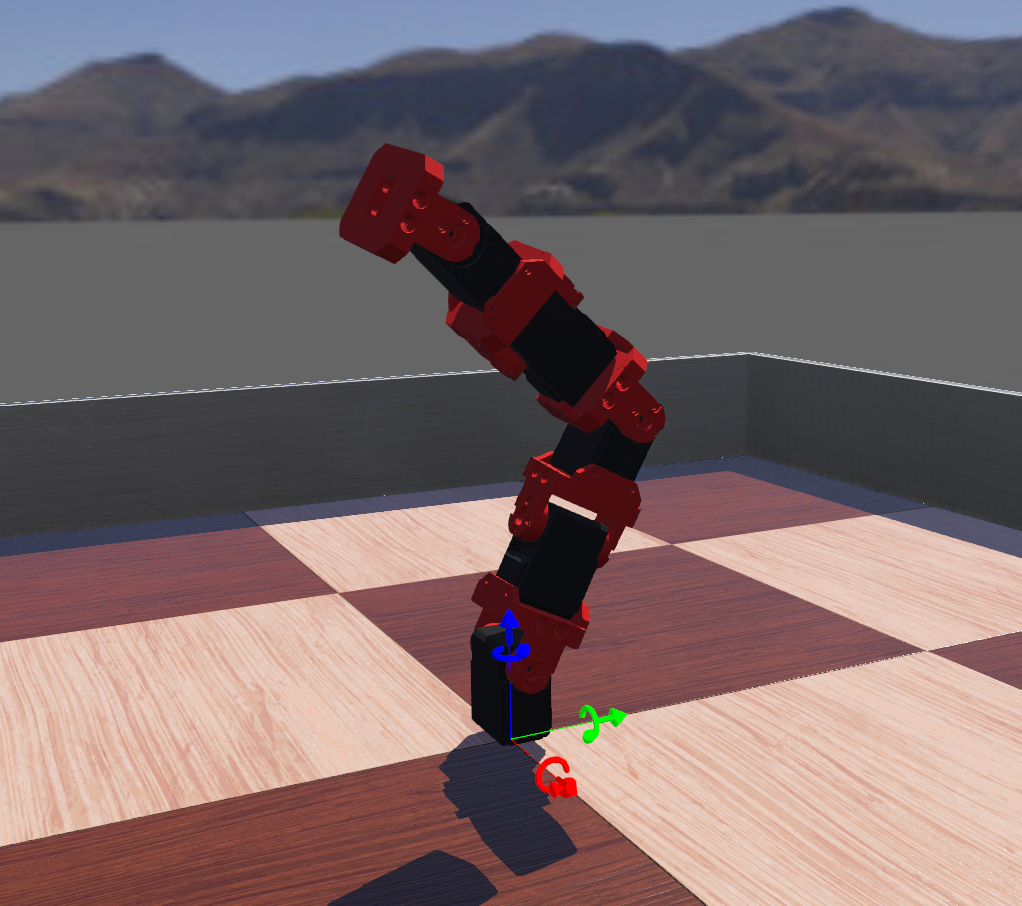
\includegraphics[width=0.8\textwidth]{./Images/webots-robot.png}
    \caption{Modelo virtual do manipulador no Webots.}\label{fig:robot-model}
\end{figure}

\subsection*{Modelagem da Cadeia Cinemática}

A estrutura cinemática do manipulador 5R foi pensada de modo a ser uma simples
cadeia de juntas rotacionais, permitindo uma fácil construção do robô real,
como por exemplo, sendo composto por uma sequência de servo motores conectados
por soquetes como ilustrado na figura~\ref{fig:robot-model}. A cadeia
cinemática é similar ao que já vimos no exemplo dos braço planar 3R, contudo
juntas consecutivas possuem eixos de rotação ortogonais entre si. Com isso, a
posição do efetuador final não fica restrita a um plano perpendicular ao eixo
de rotação das juntas, o que permite especificarmos no espaço de trabalho,
vetores com três coordenadas para compor a trajetória a ser seguida. Como \(n =
5 \text{ e } m = 3\) o manipulador tem um grau de redundância de duas juntas
excedentes. A tabela~\ref{tab:dh-parameters-5r} resume os parâmetros DH
utilizados para modelar a cadeia cinemática.

\begin{table}[htbp]
    \centering
    \begin{tabular}{c c c c c c}
        \toprule
        \textbf{Elo} & \(\theta\)   & \(d\) & \(a\) & \(\alpha\)   \\
        \midrule
        1            & \(\theta_1\) & 0     & 0.06  & \(\pi / 2\)  \\
        2            & \(\theta_2\) & 0     & 0.06  & \(-\pi / 2\) \\
        3            & \(\theta_3\) & 0     & 0.06  & \(\pi / 2\)  \\
        4            & \(\theta_4\) & 0     & 0.06  & \(-\pi / 2\) \\
        5            & \(\theta_5\) & 0     & 0.02  & \(\pi / 2\)  \\
        \bottomrule
    \end{tabular}
    \caption{Parâmetros DH para o manipulador 5R.}\label{tab:dh-parameters-5r}
\end{table}

A fixação de frames imposta pela convenção DH nem sempre permite que o frame da
base do manipulador coincida com o frame do mundo, introduzindo nesse caso a
utilização de \emph{offsets} nos parâmetros variáveis das juntas, ou
transformações fixas entre os frames que não mudam conforme as juntas são
atuadas. Optamos por adotar uma abordagem mais direta, onde introduzimos a
transformação \(\mathbf{T}^{w}_0\) que relaciona o frame do mundo \(\{w\}\) com
o frame da base do manipulador \(\{0\}\):

\begin{equation}
    \mathbf{T}^{w}_0 = Trans_z(0.04) \cdot Rot_z(\pi) \cdot Rot_y(\pi / 2)
\end{equation}

Assim, para se calcular a cinemática direta do manipulador, prosseguimos de
maneira usual na cadeia cinemática adicionando a transformação
\(\mathbf{T}^{w}_0\) ao início da multiplicação matricial:

\begin{equation}
    \mathbf{T}^{w}_5 = \mathbf{T}^{w}_0 \cdot \mathbf{T}^{0}_1 \cdot \mathbf{T}^{1}_2 \cdot \mathbf{T}^{2}_3 \cdot \mathbf{T}^{3}_4 \cdot \mathbf{T}^{4}_5
\end{equation}

Por outro lado, durante a etapa da cinemática inversa diferencial, precisamos
especificar vetores livres \(\xi^w\) que indicam a velocidade cartesiana do
efetuador no mundo em termos do frame da base do manipulador. Para isso,
utilizamos a matriz de rotação da transformação inversa (do frame \(\{0\} \to
\{w\}\)), isto é:

\begin{equation}
    \xi^0 = {Rot(\mathbf{T}^w_0)}^\top \xi^w
\end{equation}

\begin{figure}
    \centering
    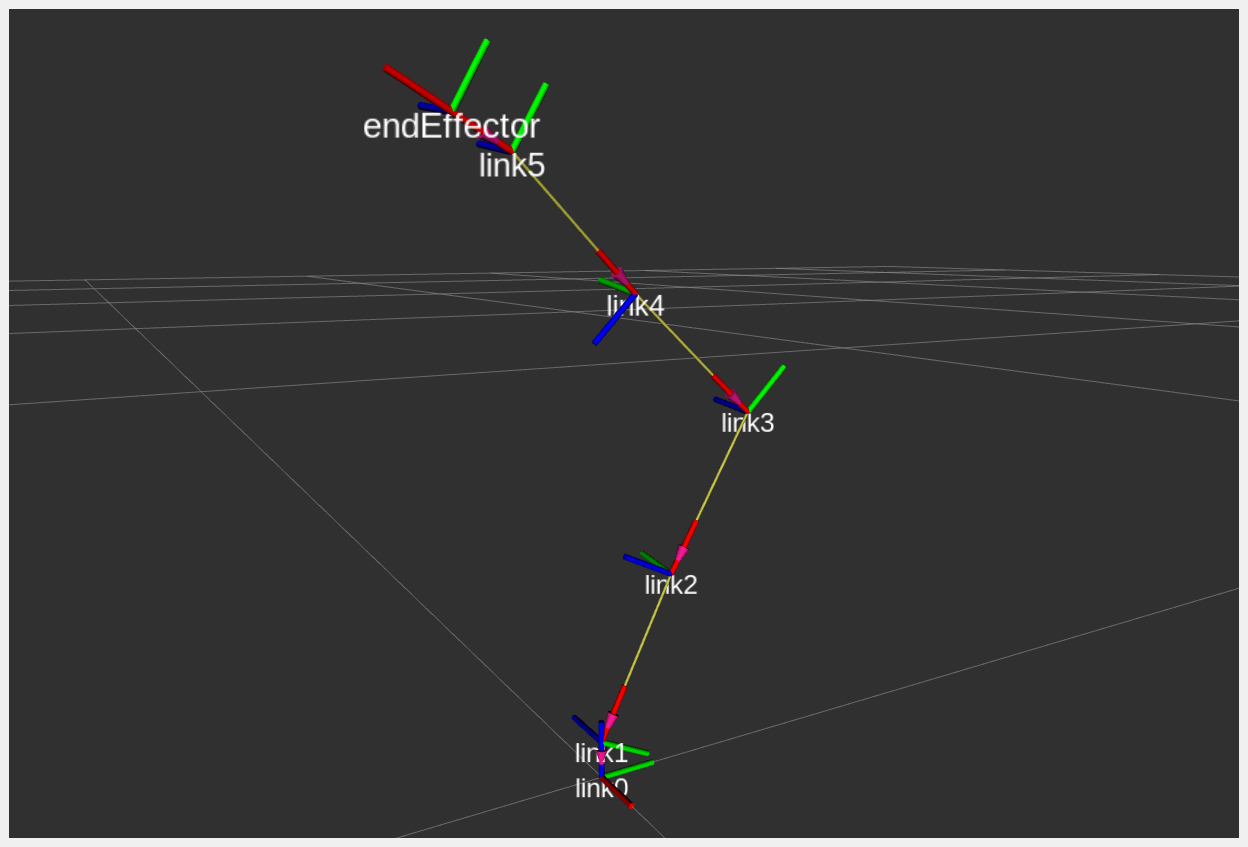
\includegraphics[width=0.8\textwidth]{./Images/rviz-chain.png}
    \caption{Cadeia cinemática visualizada no RViz.}\label{fig:kin-chain}
\end{figure}

\subsection*{Modelo dinâmico do manipulador}

Com o intuito de conferir um caráter mais realista para a simulação, um modelo
dinâmico para o robô foi construído especificando as propriedades físicas e
geometrias de colisão de cada elo no simulador. A figura~\ref{fig:dyn-chain}
mostra as formas primitivas do tipo \emph{Box} (caixas) que foram usadas para
compor a geometria de cada par servo-soquete que compõe um elo da cadeia. Para
o simulador computar o modelo dinâmico ao longo do tempo, foram fornecidas as
informações de massa do servo-motor (disponível na especificação do fabricante)
e no caso dos soquetes, a densidade do material PLA foi utilizada para estimar
sua massa com base no volume da geometria modelada (conjunto de caixas). Além
disso, a definição das matrizes de inércia ficou por conta do próprio
simulador, que estima seu valor com base na massa fornecida e na posição e
orientação das primitivas utilizadas durtante a modelagem. Vale ressaltar que a
adição das propriedades dinâmicas tem caráter apenas de aproxição de um cenário
mais real, tendo em vista que o esquema de controle proposto atua apenas na
velodidade das juntas ao passo que a posição do motor é controlada de maneira
automática pelo simulador através de um PID intrisceco à simulação de um
dispositivo como o motor.

\begin{figure}
    \centering
    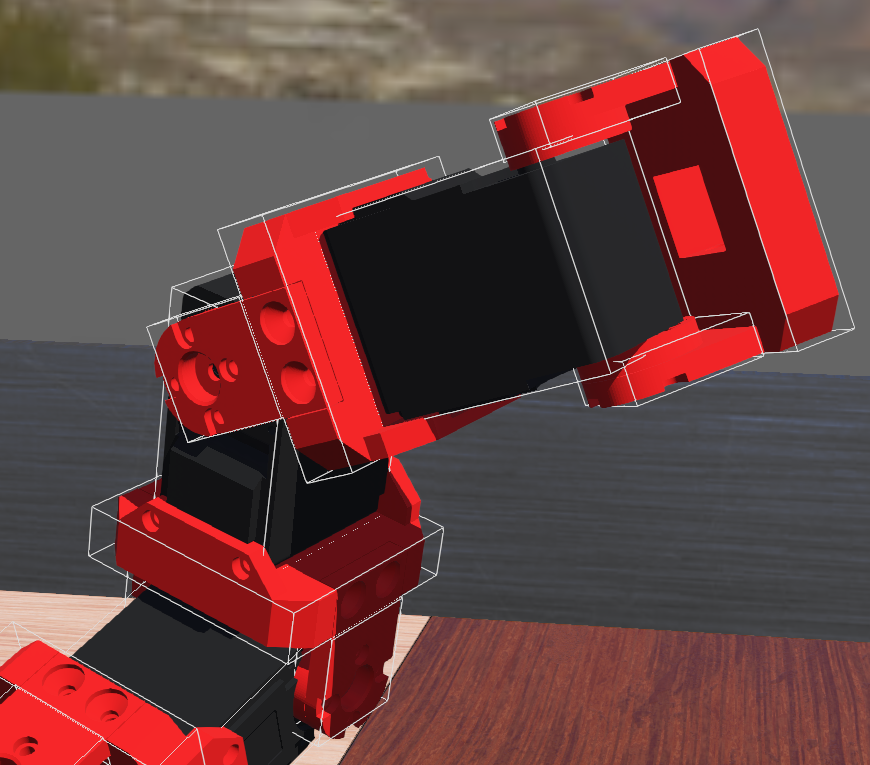
\includegraphics[width=0.6\textwidth]{./Images/dynamic-model.png}
    \caption{Geometria de colisão do modelo virtual do manipulador.}\label{fig:dyn-chain}
\end{figure}

\section{Arquitetura de comunicação}

A comunicação do controlador com o ambiente simulado do robô foi feita através
do uso do framework ROS, que consiste num conjunto de bibliotecas e pacotes de
software que facilitam a troca de mensagens entre diferentes componentes de um
sistema robótico. O próprio simulador Webots oferece suporte nativo ao ROS2,
com uma documentação detalhada de como configurar um projeto e o uso básico de
troca de mensagens entre diferentes processos.

A arquitetura do ROS2 é baseada em uma estrutura de grafo, onde nós representam
processos individuais que interagem com outros nós recebendo e enviando
mensagens, através de tópicos. Idealmente, um nó deve ser responsável por uma
única tarefa modular, como controlar os motores do robô ou enviar dados
coletados por um sensor de distância.

Os tópicos são os canais pelos quais os nós trocam mensagens e seguem um modelo
\emph{publisher/subscriber}, onde nós publicam mensagens em um tópico e outros
nós se inscrevem para receber essas mensagens, de maneira completamente
anônima. As mensagens passadas nos tópicos podem variar amplamente e geralmente
são definidas pelo usuário, cobrindo dados de sensores, comandos de controle de
motores, informações de estado, comandos de atuadores entre outros.

\subsection*{ROS2 Actions}

As ações do ROS2 expandem as capacidades do Sistema Operacional de Robôs,
proporcionando uma maneira de executar tarefas longas e orientadas a objetivos.
Ao contrário dos tópicos, que são adequados para passagem simples de mensagens,
as ações são projetadas para interações mais complexas, como mover um robô para
uma localização específica ou executar uma sequência de ações. As ações
consistem em três componentes principais: o objetivo, o resultado e o feedback.
O cliente envia um objetivo para o servidor, que então executa a ação
solicitada. Durante a execução, o servidor pode fornecer feedback ao cliente
para mantê-lo informado sobre o progresso. Uma vez concluída a ação, o servidor
envia um resultado de volta ao cliente. Este padrão de comunicação assíncrona
permite o manuseio robusto de tarefas que podem levar algum tempo para serem
concluídas, proporcionando melhor controle e monitoramento do sistema como um
todo. As ações do ROS2 são uma ferramenta poderosa para construir aplicativos
robóticos avançados, permitindo que os robôs executem tarefas complexas com
precisão e eficiência.

\subsection*{Grafo de comunicação no ROS2}

A arquitetura de comunicação proposta para o controle do manipulador é
ilustrada no grafo da figura~\ref{fig:coms_arch}, onde temos nós, tópicos e
ações associados a execução de uma trajetória. A seguir temos uma breve
descrição do funcionamento de cada nó:

\begin{itemize}
    \item \textbf{snake\_driver} {-} Nó instânciado pelo simulador responsável por controlar os motores do manipulador.
          Está inscrito no tópico \texttt{target\_joint\_states} que recebe a configuração das juntas desejada para o manipulador
          e publica no tópico \texttt{joint\_states} os valores lidos pelos sensores de posição de cada motor. Este nó pode ser substuído por um nó
          que se comunique com um robô real, bastando que a interface de comunicação seja mantida, garantindo uma transferência natural do ambiente simulado para testes físicos.

    \item \textbf{snake\_controller} {-} Nó responsável por implementar a lógica de controle do manipulador. Este nó está inscrito/publica nos dois tópicos
          \texttt{target\_joint\_states} e \texttt{joint\_states} anteriores para interação com o \emph{driver} do manipulador. Além disso, se inscreve
          num tópico \texttt{rrc\_input}, recebendo parâmetros de controle do algoritmo~\ref{rrc-alg} e publica no tópico \texttt{rrc\_output} dados
          relativos à posição do efetuador final e métricas de desempenho.

    \item \textbf{trajectory\_action\_server} {-} Nó responsável por receber um objetivo de posição e informações do efetuador final para execução de uma trajetória
          no espaço de trabalho do manipulador, publicando no tópico \texttt{rrc\_input} os parâmetros de controle.

    \item \textbf{trajectory\_action\_client} {-} Nó responsável por enviar um objetivo de posição para o servidor de ação \texttt{trajectory\_action\_server} e
          receber o resultado da execução da trajetória. Através da interface de ação, o cliente recebe feedback do progresso da execução da trajetória e o resultado final,
          salvando todos os dados em um arquivo de \emph{log}, para posterior análise.
\end{itemize}

\begin{figure}
    \centering
    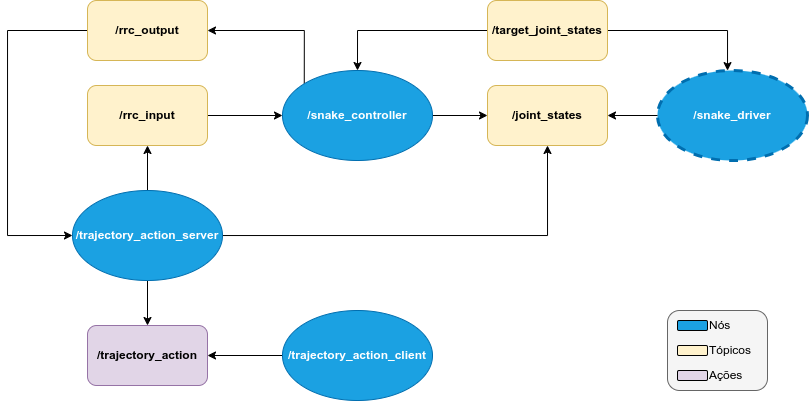
\includegraphics[width=0.9\textwidth]{./Images/com-arch.png}
    \caption{Arquitetura de comunicação proposta para controle do manipulador.}\label{fig:coms_arch}
\end{figure}

\section{O Algoritmo \emph{Resolved Rate Control}}

\begin{figure}
    \centering
    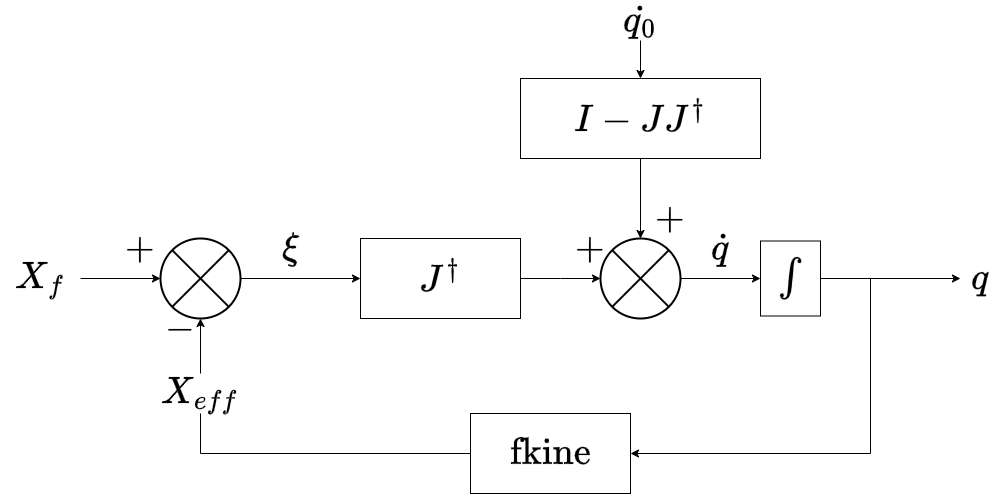
\includegraphics[width=0.9\textwidth]{./Images/control-scheme.png}
    \caption{Diagrama de blocos do controlador RRC}\label{fig:block-diagram}
\end{figure}

\begin{algorithm}
    \caption{\emph{Resolved Rate Controller} {-} Atualizando o estado das juntas}\label{rrc-alg}
    \begin{algorithmic}[1]\Procedure{updateJointPosition}{$q$, $\xi$, $k_0$, $\delta_t$, \texttt{metricName}}
        \State$\xi \gets {Rot(\mathbf{T}^w_0)}^\top \xi$
        \State$J \gets Jacobian(q)$
        \State$J^\dag \gets J^\top {(J J^\top)}^{-1}$

        \State$n \gets length(q)$
        \State$\dot{q_0} \gets array(size: n)$

        \For{$i \gets 0 \ \texttt{to} \ n - 1$} \Comment{Calculando o gradiente da métrica}
        \If{$\texttt{metricName} = \texttt{joint\_distance}$}
        \State$q_{mid} \gets 0.5 \times (q_{\max}[i] + q_{\min}[i])$
        \State$\dot{q_0}[i] \gets (-k_0 / n) \times (q[i] - q_{mid}) \div {{(q_{\max}[i] - q_{\min}[i])}^2}$
        \ElsIf{$\texttt{metricName} = \texttt{manipulability}$}
        \State$q_{+} \ , \ q_{-} \gets copy(q) \ , \ copy(q)$
        \State$q_{+}[i] \gets q_{+}[i] + h$
        \State$q_{-}[i] \gets q_{-}[i] - h$
        \State$\dot{q_0}[i] \gets k_0 \times (manipulability(q_{+}) - manipulability(q_{-})) \div (2 \times h)$
        \EndIf{}
        \EndFor{}

        \State$\dot{q} \gets J^\dag \xi + (I - J^\dag J) \dot{q_0}$

        \State\textbf{return} $clipLimits(q + \dot{q} \delta_t, q_{\max}, q_{\min})$ \Comment{Restringe aos limites das juntas}
        \EndProcedure\end{algorithmic}
\end{algorithm}

\section{Experimentos}

cenário 1 -> q0 == qf (variação de métrica controla o tempo de execução)

cenário 2 -> q0 != qf (erro da posição e variação de métrica controla o tempo
de execução)

cenário 3 -> q0 != qf com q0 ~ N(0, 0.1) (erro da posição e variação de métrica
controla o tempo de execução) repetir 100x

\begin{figure}
    \centering
    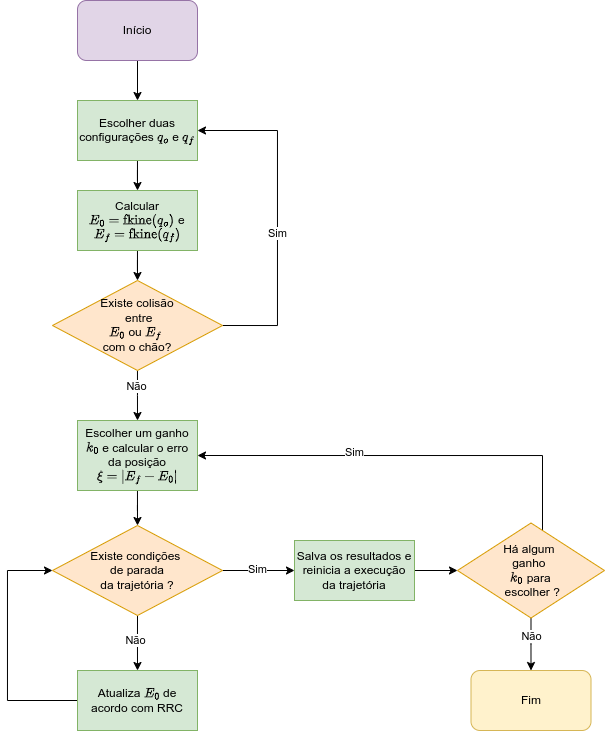
\includegraphics[width=0.8\textwidth]{./Images/exp-flow.png}
    \caption{Etapas seguidas em cada execução de uma \textbf{trajectory\_action}.}\label{fig:exp-flow}
\end{figure}

